%\documentclass[12pt]{article}
%\usepackage{amsmath}
%\usepackage{graphicx, color}
%\usepackage{amssymb}
%\usepackage{listings} %source code listing
%\usepackage{multirow}
%%\usepackage[version=2]{mhchem}
%\usepackage{subfig}
%\usepackage{hyperref}
%\usepackage{units}
%\usepackage{gensymb}
%\usepackage{adjustbox}
%\usepackage{listings}
%\usepackage{color}
%\usepackage{tcolorbox}
% 
%\definecolor{codegreen}{rgb}{0,0.6,0}
%\definecolor{codegray}{rgb}{0.5,0.5,0.5}
%\definecolor{codepurple}{rgb}{0.58,0,0.82}
%\definecolor{backcolour}{rgb}{0.95,0.95,0.92}
%
%\newcommand{\specialcell}[2][c]{%
%  \begin{tabular}[#1]{@{}c@{}}#2\end{tabular}}
% 
%
%
%\title{Reactor physics with Python \\ Lecture Notes}
%
%
%\author{Zs.~Elter. E. Branger, M. Preston \\ Uppsala University \\
%        Division of Applied Nuclear Physics}%\corref{cja}}
%%
%\date{2021.}
%\begin{document}

\section{Appendix}

\subsection{Solid angle}

When describing the movement of neutrons, it is often not only the speed of neutrons but also the velocity $\mathbf{v}$ of neutrons which is of interest. Nevertheless, instead of handling the velocity directly, it is rather the energy $E$ and the direction unit vector $\mathbf{\Omega}$:

\begin{equation}
\mathbf{\Omega}=\frac{\mathbf{v}}{|\mathbf{v}|}=\mathbf{e_x}\sin\theta\cos\phi+\mathbf{e_y}\sin\theta\sin\phi+\mathbf{e_z}\cos\theta
\end{equation}

\noindent where we introduce the spherical space coordinates, the polar angle $\theta$ and the azimuthal angle $\phi$. 

\begin{figure}[ht!]
\protect \centering{
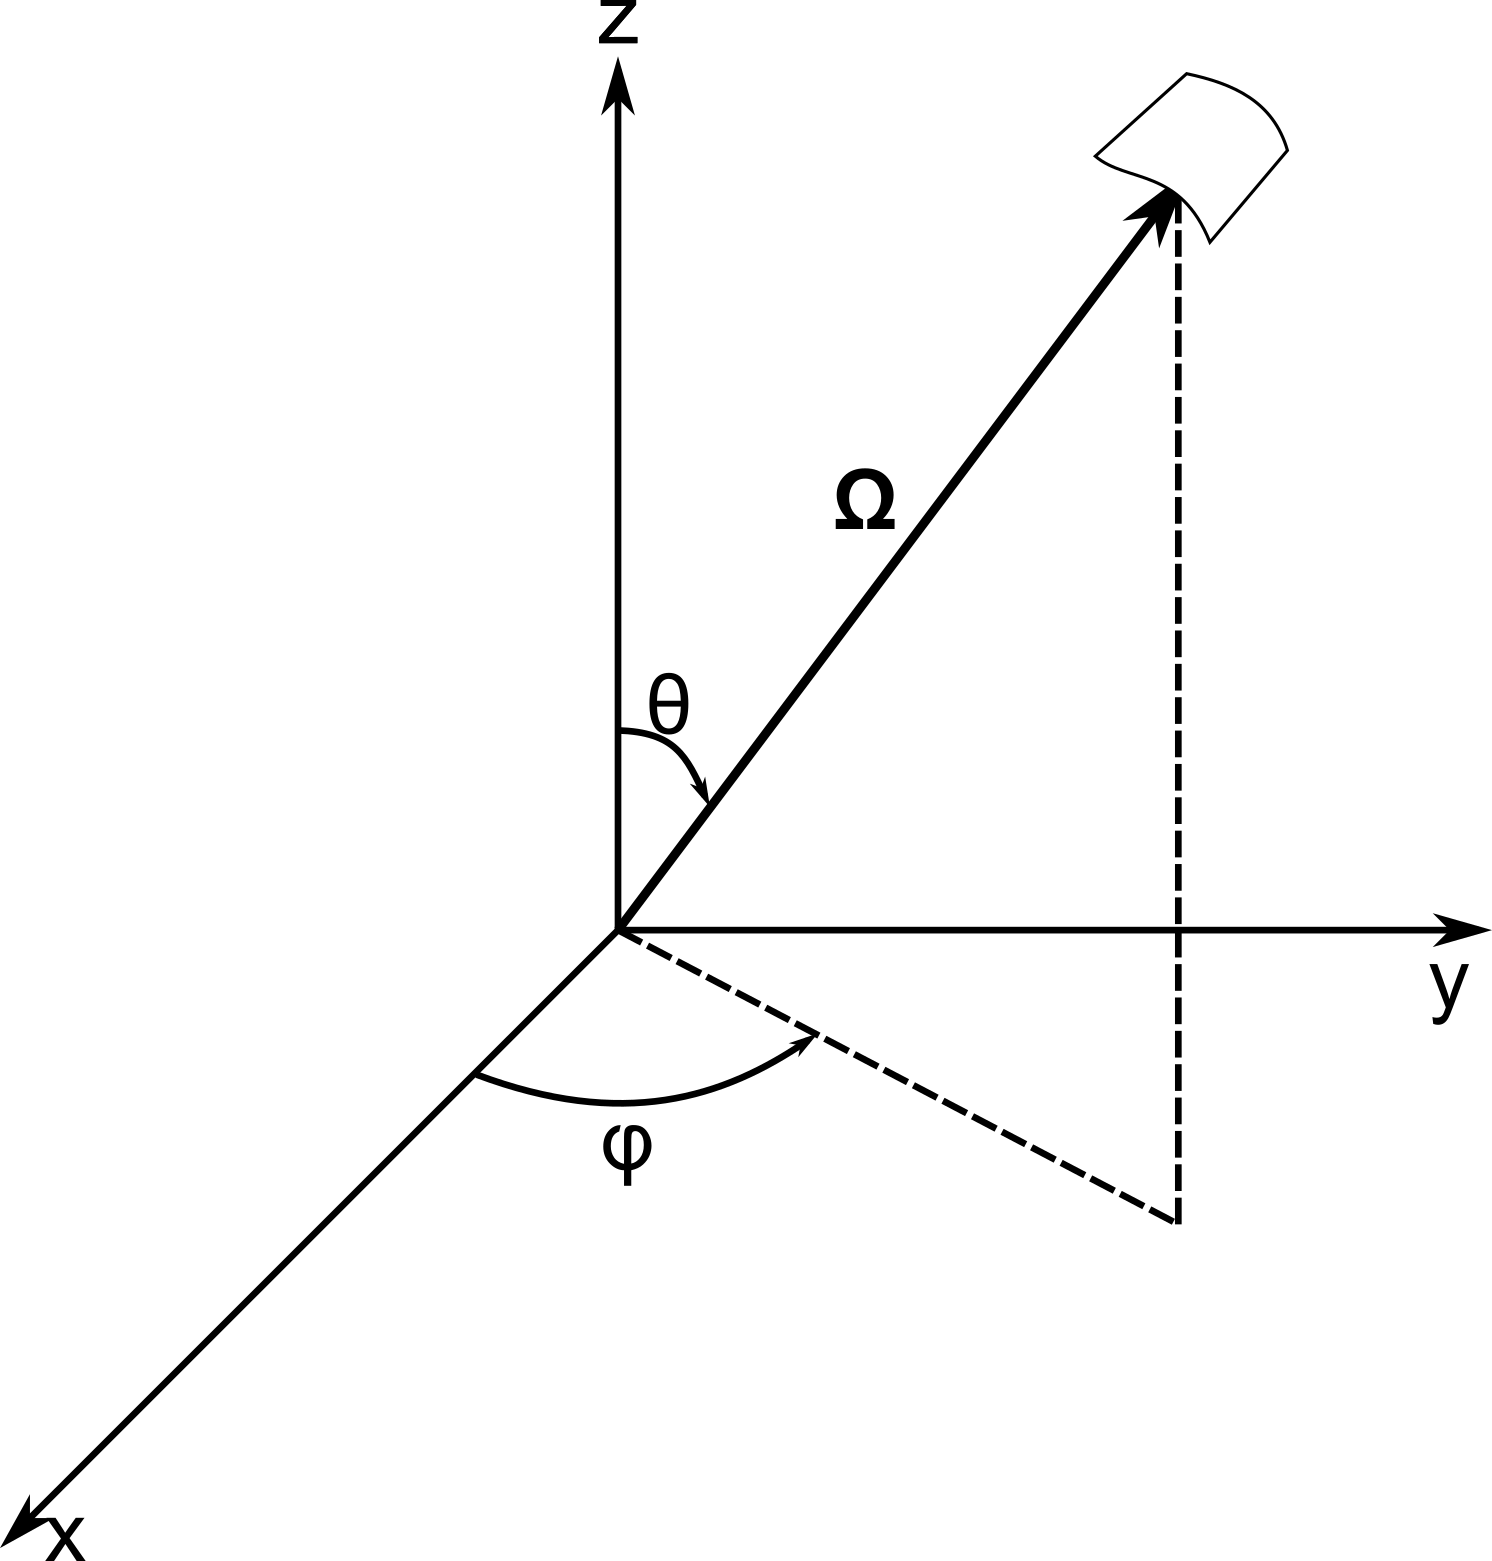
\includegraphics[scale=0.44] {figures/A-solidangle.png}}\protect
\caption{\label{fig:solidangle} \footnotesize{Representation of direction and solid angle.}}
\end{figure}

Thus when integrating a function over velocity, we can substitute

\begin{equation}
\int f(\mathbf{v})d^3v=\int\limits_0^\infty v^2 dv\int\limits_0^{2\pi}d\phi\int\limits_0^\pi \sin\theta f(\mathbf{v})d\theta
\end{equation}

\noindent and we can further define that 

\begin{equation}
\int\limits_{4\pi}d\mathbf{\Omega}=\int\limits_0^{2\pi}d\phi\int\limits_0^\pi \sin\theta d\theta
\end{equation}

\noindent and we can notice that in fact the differential $d\mathbf{\Omega}$ is a solid angle (an area illustrated with the small patch in Figure \ref{fig:solidangle})

\[
d\mathbf{\Omega}=\sin\theta d\theta d\phi
\]

We will frequently encounter integrals over this small solid angle.


\subsection{Monte Carlo methods}

Monte Carlo methods provide a direct solution to the transport equation, since it allows for faithful simulation of neutron trajectories while they move around in matter. Of course it still means that we need to implement the correct physics (for example scattering kernel), and have the right cross sections, but we do not need to discretize space, angle or energy. Thus, the geometry can be arbitrarily complex and handled in 3D.

The idea is that one tracks neutrons as from birth to death, and randomly samples the collisions and the locations of the collisions the neutron enters. If one could simulate every neutron than the accuracy would be the same as performing a measurement. Nevertheless, due to the lack in computational power, usually we are not able to simulate every neutron, therefore our results (k-eff,  reaction rates, flux) will be average over the population of neutrons sampled. An other source of accuracy in this methods comes from the uncertainty in the measured cross section data, which propagates into the Monte Carlo simulations.

Covering Monte Carlo particle transport could be in itself a full course, so here we cover only some very basic ideas we will be using. In order to faithfully simulate neutrons, we will need

\begin{itemize}
\item To implement physics (for example scattering kernels)
\item Sample coordinates, angles, reactions, energies. So in general: sample probability density functions
\item Track neutrons and perform coordinate transformations.
\end{itemize}


Therefore, in this Appendix we briefly review pseudo random numbers, and  probability density functions sampling.

\subsubsection{Random numbers}

In order to sample probability density functions, we need random numbers. What is random? Something which lacks pattern and predictability. It doesn't make sense to discuss the randomness of a single number or event, only for a sequence of number of events. There are several methods to decide whether a sequence of numbers can be considered random.

One could use measurement of random fluctuations of nature to generate random numbers. But this needs the data to be tabulated. Similarly we could use irrational numbers, such as $\pi$ as shown in Fig. \ref{fig:randompi}. In several applications in fact such tabulated data is being used.

\begin{figure}[ht!]
\protect \centering{

\includegraphics[scale=0.44] {figures/randomized_pi_rect.png}}\protect
\caption{\label{fig:randompi} \footnotesize{The digits of $\pi$, each digit 0-9 is assigned to a different color.}}
\end{figure}


However, it is often more practical to use a computer to generate random numbers. Now of course a computer is deterministic, so these will only be \textit{pseudo random numbers}. The great advantages is, that if using the same seed, we can get the same sequence, which is useful for tests and debugging. 

For example a simple algorithm to generate pseudo random numbers can be $X_{n+1}=\text{k middle digit of }\: X_n^2$. But algorithms like that will have a period (once the middle digits repeat we will reproduce the same sequence of numbers over and over again). A slightly improved algorithm:

\[
X_{n+1}=(aX_n+c)\%m
\]

\noindent for example with $a=1664525$, $c=1013904223$, $m=2^{32}$. This will produce longer periods.

Nevertheless, we don't need to worry about about pseudo random numbers, since for our applications the basic pseudo random number generators of numpy will be perfect.

\subsubsection{discrete distributions}

Consider we have three events with the following probabilities:


\begin{table}
\centering\begin{tabular}{c | c}
event & probability \\
\hline
A & 0.6 \\
B & 0.3 \\
C & 0.1 
\end{tabular}
\end{table}


In order to sample random events from this distrubution we can follow the algorithm in Fig. \ref{fig:discrete}, which can be generalized for cases when there are more possible events. We perform the cumulative sum of probabilities, and get event j if $\sum_{i=1}^{j-1}p_i\leq r <\sum_{i=1}^{j}p_i$

\begin{figure}[ht!]
\protect \centering{
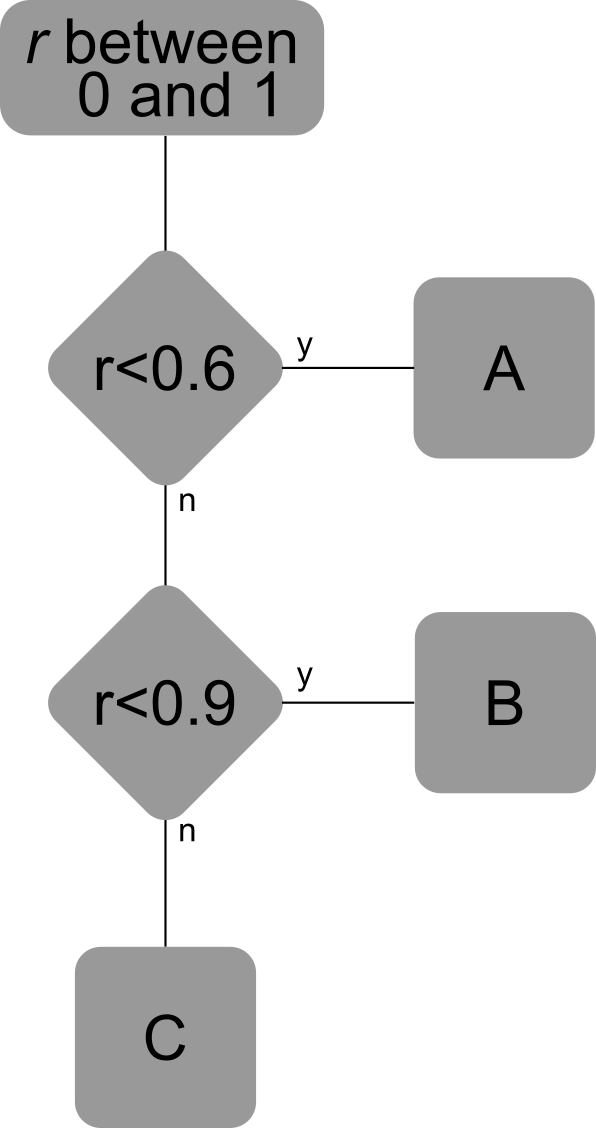
\includegraphics[scale=0.44] {figures/discreterandom.png}}\protect
\caption{\label{fig:discrete} \footnotesize{Algorithm to sample discrete events.}}
\end{figure}


In neutron transport, such discrete events will be important when we need to decide which reaction is going to happen with a neutron (with a probability $\Sigma_i/\Sigma_t$, or when we want to sample the number of neutrons emitted in a fission event. 

\subsubsection{Sampling continuous distributions}

Let's consider that the distribution of a random value $x$ is described by a probability density function $p(x)$, and the related cumulative distribution function is $F(x)=\int_{-\infty}^xp(t)dt$ as shown in Fig. \ref{fig:pdfcdf}

\begin{figure}[ht!]
\protect \centering{
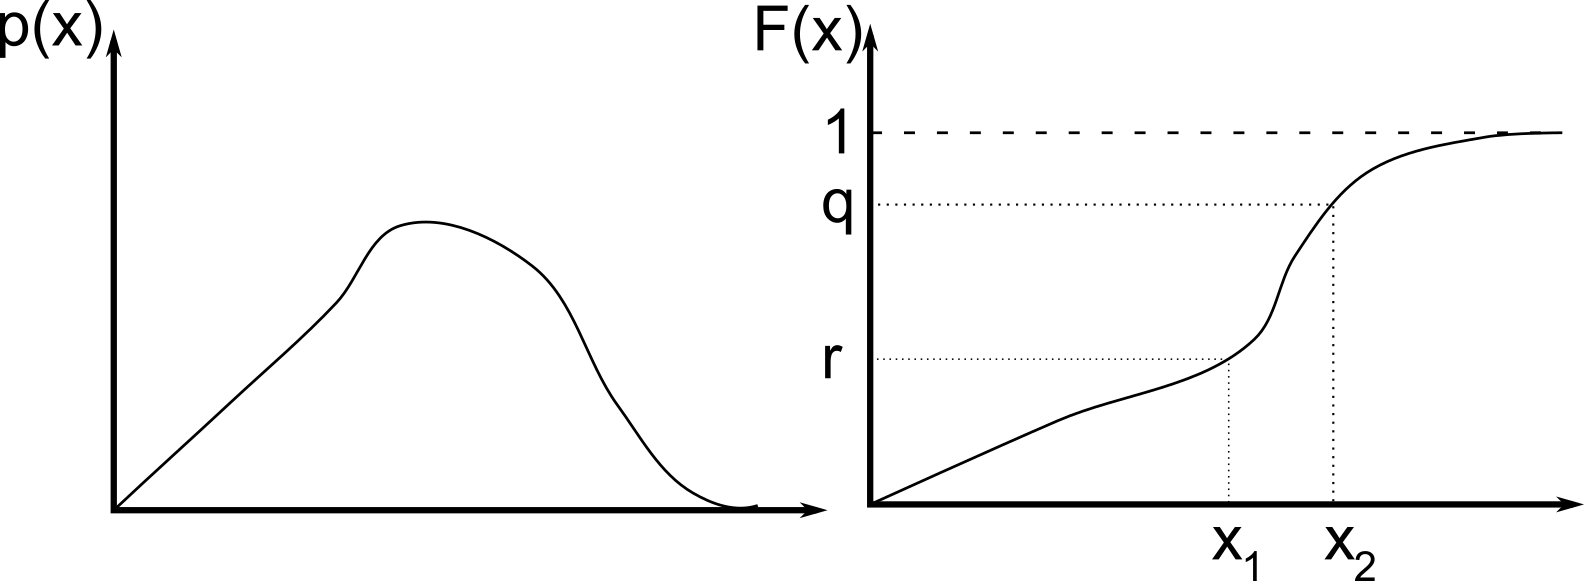
\includegraphics[scale=0.44] {figures/cont_distr1n.png}}\protect
\caption{\label{fig:pdfcdf} \footnotesize{Illustration of a probability density function and the related cumulative distribution function.}}
\end{figure}

The cumulative distribution function is going to take values between 0 and 1. So if one can have uniformly distributed random numbers between 0 and 1, it is possible to convert the random number $r$ to get a random value $x$:

\[
x=F^{-1}(r)
\]


This method can be applied however only, when it possible to easily integrate the probability density function. This is for example the case in neutron transport when we need to sample random distances between collisions, since as we saw before, the distribution of the distance between collisions follows an exponential distribution. 

However, if the given distribution is less well-behaving, and it is difficult to obtain the cumulative distribution function, we still have several options, from which here we review only one, the so called rejection sampling. We draw a random number, convert it to be between a and b, we draw an other one to create a y value based on the maximum of the pdf. If we are under the curve we accept the value, otherwise we reject it, and draw a new number. The algorithm is summarized in Fig. \ref{fig:rejection} Such a method will be useful, when for example sampling the birth neutron spectrum.

\begin{figure}[ht!]
\protect \centering{
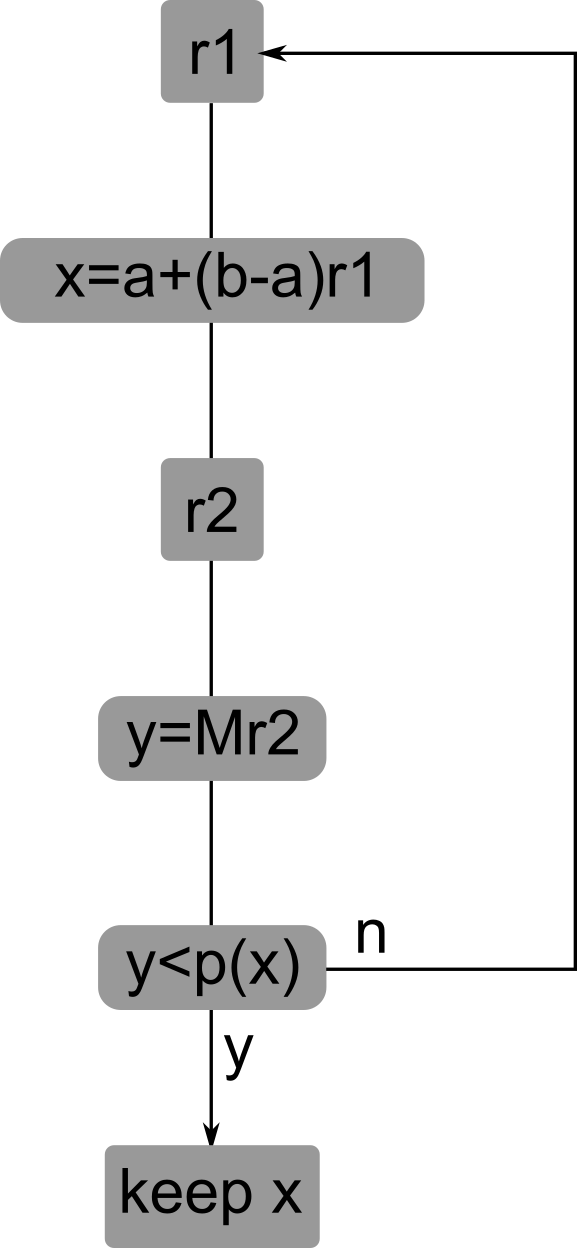
\includegraphics[scale=0.44] {figures/rejection.png}}\protect
\caption{\label{fig:rejection} \footnotesize{Algorithm of rejection based sampling.}}
\end{figure}

\subsubsection{Coordinates after scattering}

During elastic scattering we derived that both the energy and the direction of the neutron is going to change, and we saw that there is a connection between the two. Usually we will sample the new energy from the scattering kernel, and use it to figure out the scattering angle. However, then we still need to update the direction of the neutron. For transforming the directions we can use the following formulae (from \url{https://docs.openmc.org/en/v0.10.0/methods/physics.html}), which is based on coordinate transformation considerations not derived here.

\begin{equation}
u' = \mu u + \frac{\sqrt{1 - \mu^2} ( uw \cos\phi - v \sin\phi )}{\sqrt{1 -
w^2}} 
\end{equation}
\begin{equation}
v' = \mu v + \frac{\sqrt{1 - \mu^2} ( vw \cos\phi + u \sin\phi )}{\sqrt{1 -
w^2}} 
\end{equation}
\begin{equation}
w' = \mu w - \sqrt{1 - \mu^2} \sqrt{1 - w^2} \cos\phi
\end{equation}

%\end{document}